\documentclass[a4paper,12pt,twoside,openright]{memoir}

\newcommand{\subject}{From Existing Software to Models}

%%%% PACKAGES %%%%

\usepackage[T1]{fontenc}
\usepackage[utf8]{inputenc}
\usepackage{fourier}
\usepackage[english]{babel}

\usepackage{graphicx}
\graphicspath{{Images/}}

\begin{document}

\chapter{Process Analyse}

    \section{Beskrivelse - Hvad gjorde vi i P1} 

        \subsection{Projektplanlægning}
            Der blev lavet undervejs to tidsplaner, med deadlines til f.eks. hvornår vi skulle afslutte problemanalysen. Da ikke alle tidspunkter var realistiske under hele forløbet, blev der lavet en ny iteration.

            Der har ikke været en person, der blev udpeget at været projektleder, istedet har vi været meget demokratiske. Tilsidst i projekt forløbet tog nogle gruppemedlem rollen, som projektleder for en dag, hvis rolle var at skulle styr på hvad der var lavet og hvad der stadig manglede at blivet lavet. Beslutninger har været mere enstemmige, men beslutningerne har også først været taget efter længere diskussioner.

            \begin{figure}[ht!]
                \centering
                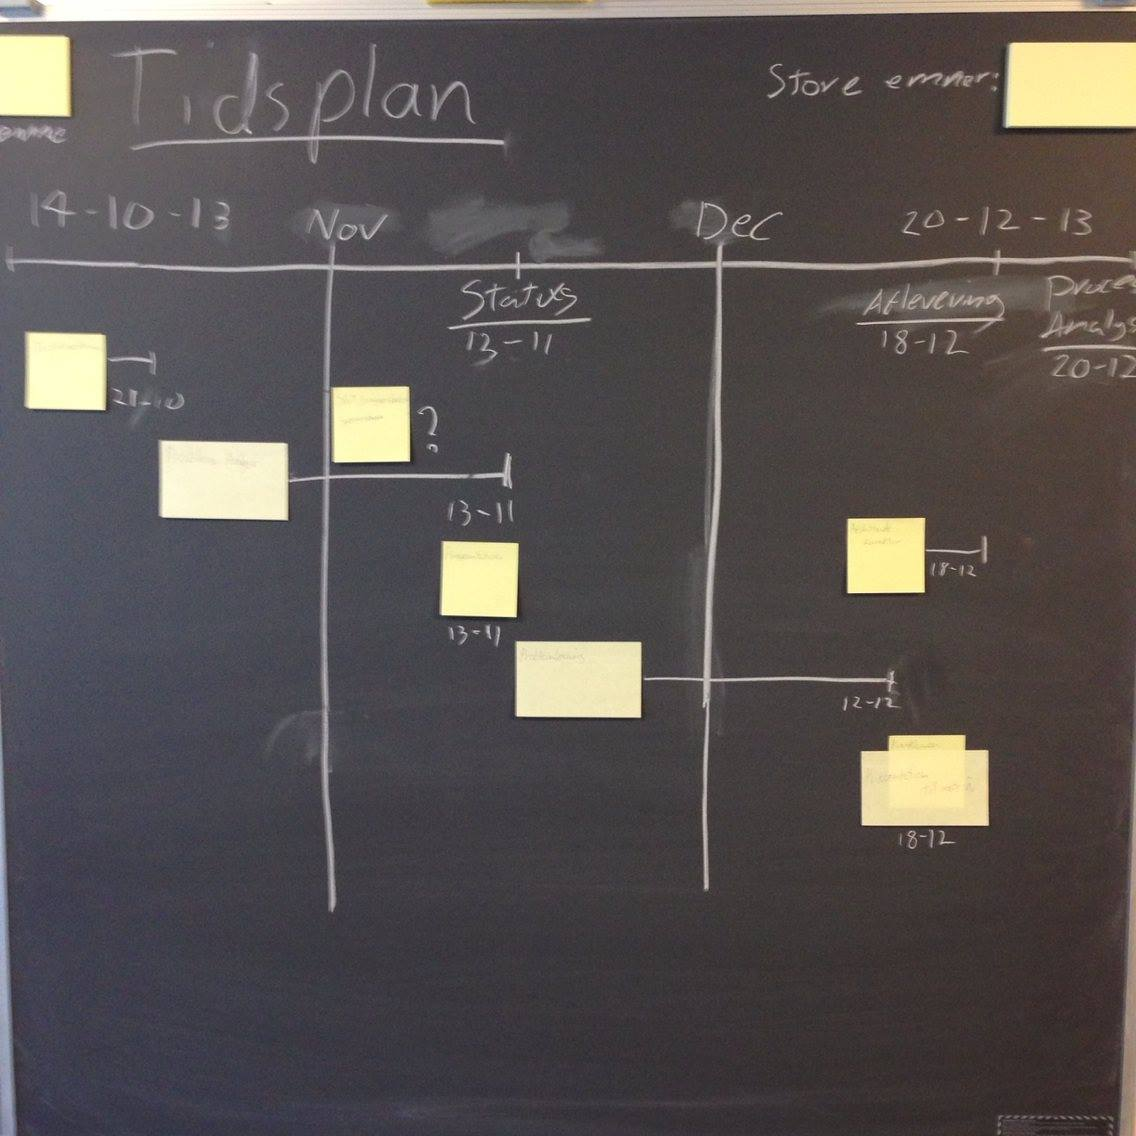
\includegraphics[width=0.5\textwidth]{Images/9.jpg}
                \caption{BAH}
                \label{4}
            \end{figure}

            \begin{figure}[ht!]
                \centering
                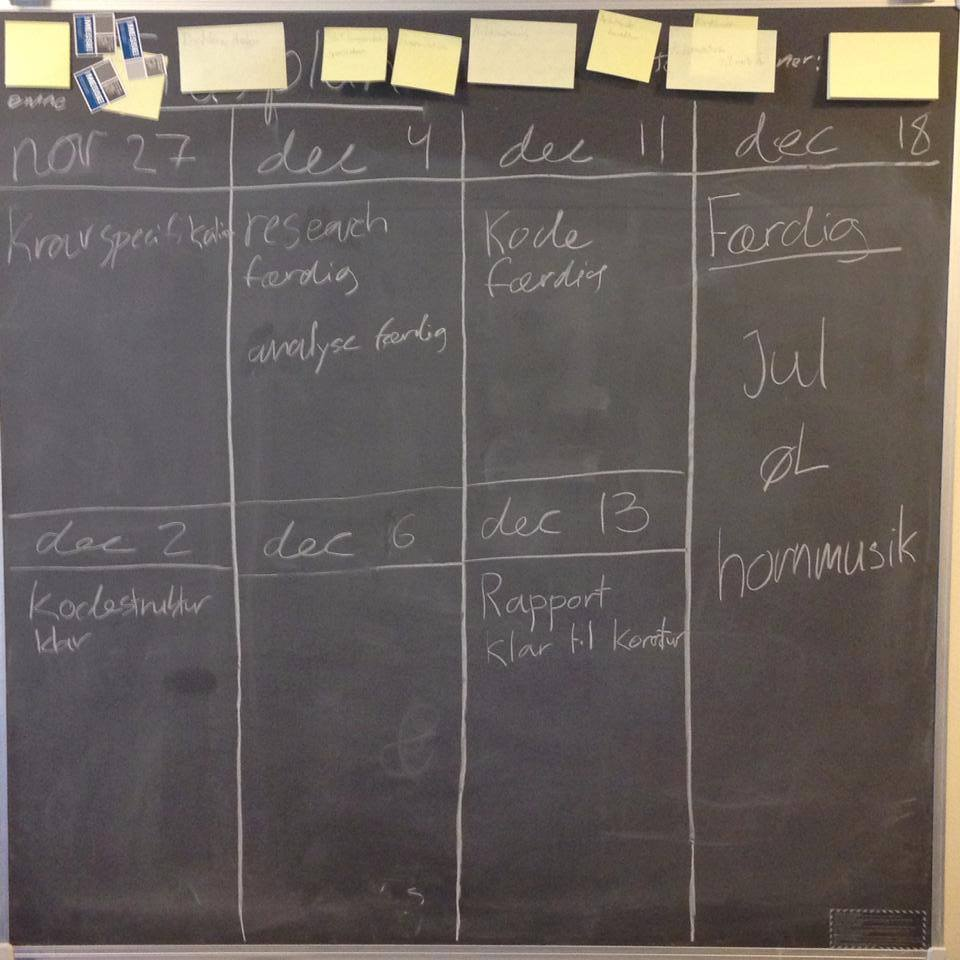
\includegraphics[width=0.5\textwidth]{Images/2.jpg}
                \caption{BAH}
                \label{4}
            \end{figure}

        \subsection{Gruppesamarbejde}
            
           %indsæt input

        \subsection{Samarbejde med vejlederen}
        Har I haft en samarbejdsaftale med jeres vejleder? I så fald: har den fungeret tilfredsstillende? 
        Hvordan forberedte I møder med jeres vejleder? 
        Hvilken type vejledning ønskede I fra vejlederen? Hvilken type vejledning fik i?  

        \subsection{Problemformuleringer}
        Hvordan lavede I indledning til problemformuleringen?
        Hvilken argumentation brugte I for at motivere problemformuleringen?
        Hvad har I lært om hvordan problemformuleringer udarbejdes?

        \subsection{Rapportstrukturering}
        Hvordan bestemte I hvilke afsnit der skulle være i jeres P0 rapport?
        Hvordan bestemte I strukturen i rapporten?
        Hvordan sikrede I en rød tråd i rapporten?
        Hvilke afsnit havde I i jeres rapport, som I mener er generelle for alle projekter?

    \section{Vurdering - Hvordan gik det}
    Når I er færdige med at beskrive hvad I gjorde, skal I vurdere hvordan det gik. Med andre ord: Hvad gik godt i P0? Hvad gik dårligt i P0? 

    \section{Analyse - Hvorfor gik det som det gik}
    Dernæst skal I analysere jeres arbejdsprocesser og få klarlagt hvorfor noget gik godt mens andet gik dårligt. Med andre ord: Hvad er det for faktorer, som har indvirket på arbejdsprocesserne? 

        \subsection{Brainstorm}
        I starten af forløbet, lavede i brainstorm på tavlen, hvor vi delte det op i 3 store  emner, "Indoor navigation", "Problemer der skal håndteres" og "Intressenter". Disse emner blev delt ind i under emner, hvor vi smed relevante problemer og emner op omkring navigation eller SOTA som kan buges til navigation. 

        \begin{figure}
        \centering
            \begin{minipage}{0.45\textwidth}
                \centering
                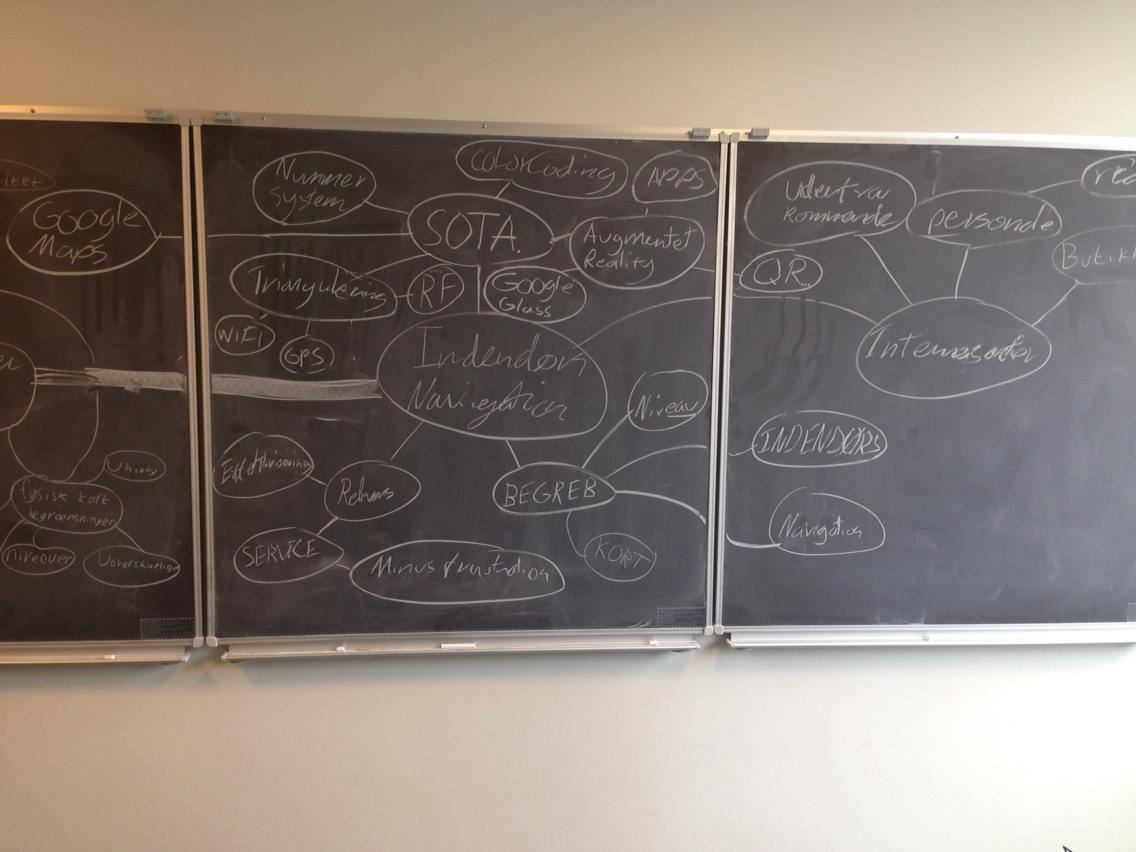
\includegraphics[width=\textwidth]{Images/1.jpg}
                \caption{BAH}
                \label{4}
            \end{minipage}
            \begin{minipage}{0.45\textwidth}
                \centering
                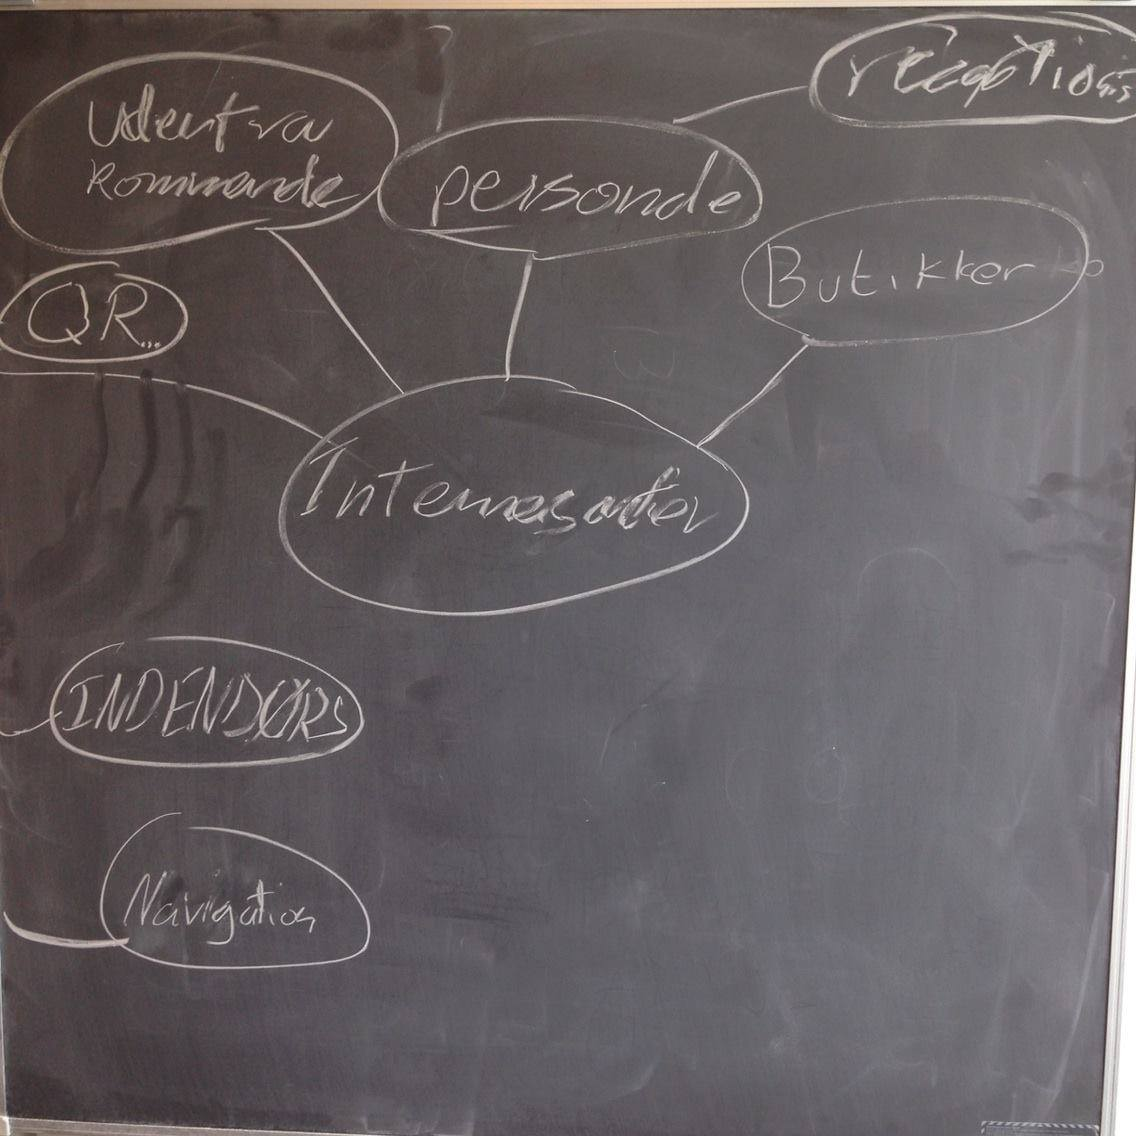
\includegraphics[width=\textwidth]{Images/3.jpg}
                \caption{BAH}
                \label{4}
            \end{minipage}
            \begin{minipage}{0.45\textwidth}
                \centering
                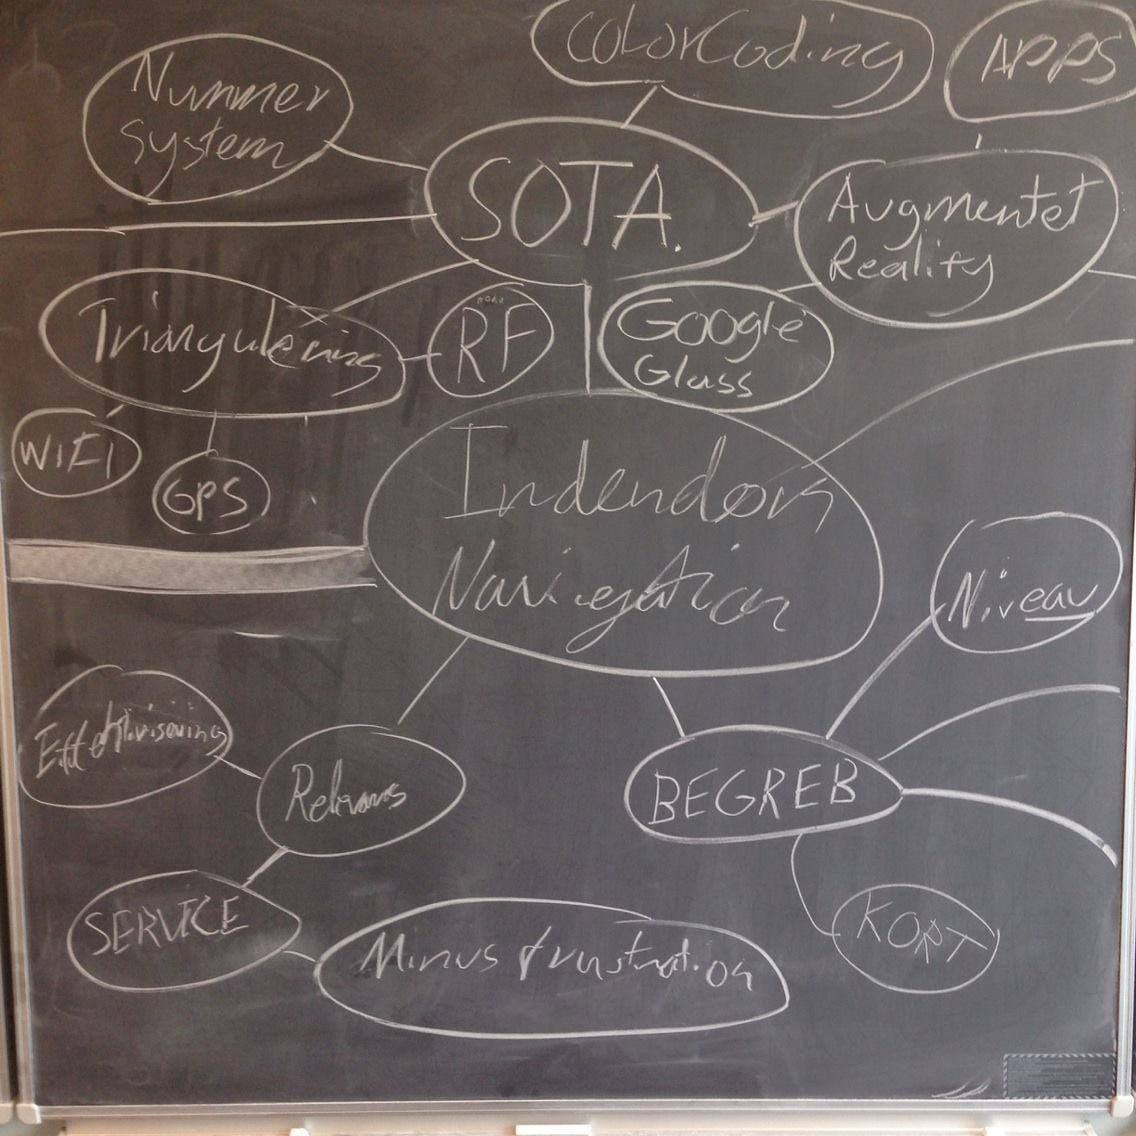
\includegraphics[width=\textwidth]{Images/4.jpg}
                \caption{BAH}
                \label{4}
            \end{minipage}
            \begin{minipage}{0.45\textwidth}
                \centering
                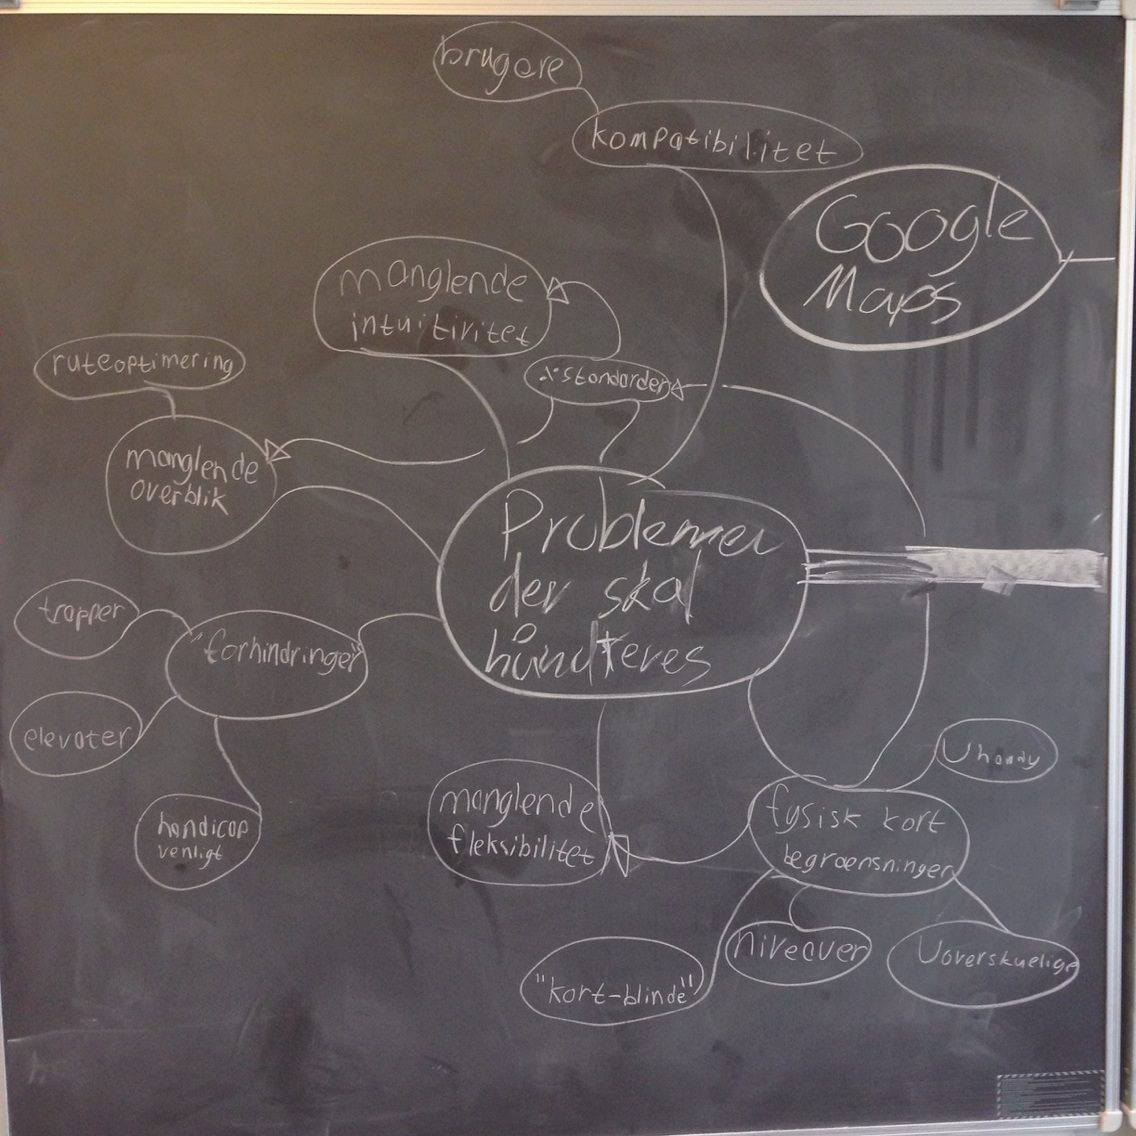
\includegraphics[width=\textwidth]{Images/7.jpg}
                \caption{BAH}
                \label{4}
            \end{minipage}
        \end{figure}

        \subsection{Tegninger}
        Under mange af vores diskussioner, har vi illustreret det for gruppen på tavlen, så alle kunne være  med og her er et af ex. på vores diskussion omkring håndtering af "Floors", der er blevet lavet mange gode ting på tavlen, men ikke alle ting er der blevet taget billeder af.

        \begin{figure}[ht!]
            \centering
            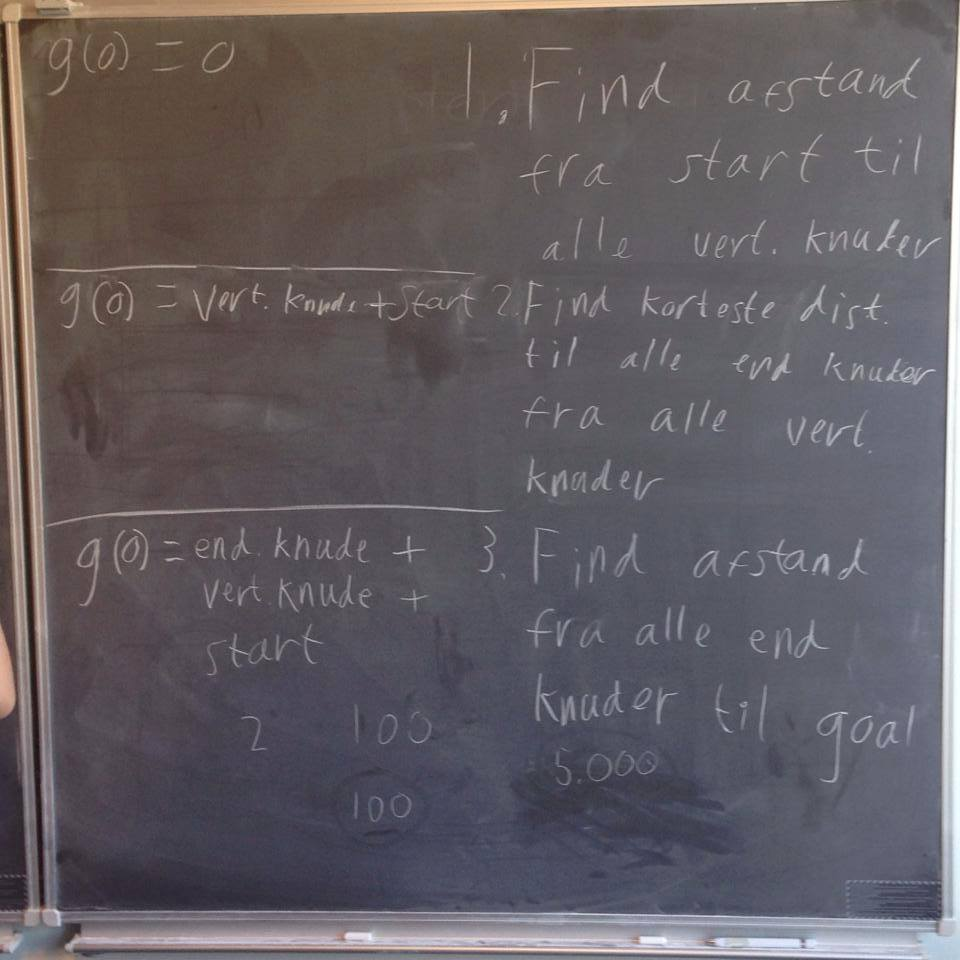
\includegraphics[width=0.5\textwidth]{Images/5.jpg}
            \caption{BAH}
            \label{4}
        \end{figure}

        \begin{figure}[ht!]
            \centering
            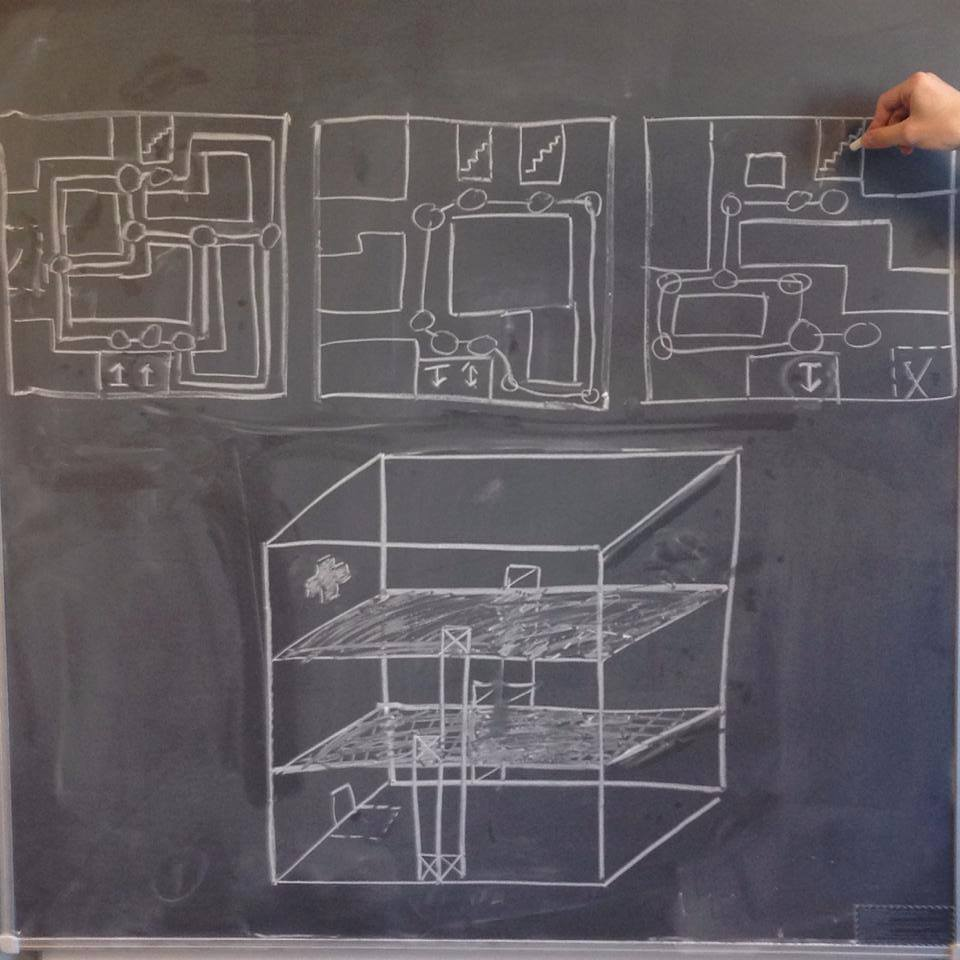
\includegraphics[width=0.5\textwidth]{Images/6.jpg}
            \caption{BAH}
            \label{4}
        \end{figure}

        \subsection{Andet}
        Under materialle læsning, sendte vi en gruppe ud på Syghus Nord Aalborg, for at tage billeder af hvordan navigeringen foregik, såsom farve kode, kort og skilte.

    \section{Syntese - Gode råd til P2}
    Hvis jeres vurdering og analyse skal bidrage til at forbedre jeres evne til at håndtere det 
    problemorienterede og projektorganiserede gruppearbejde, skal I til slut konkretisere jeres 
    erfaringer i nogle ’Gode råd’ til jer selv og jeres medstuderende. En god måde at formulere sådanne 
    gode råd på er som en *start-stop-fortsæt*-liste, dvs. en liste med følgende tre sektioner: 
    Dette vil vi begynde at gøre i P1, som vi ikke gjorde i P0 
    Dette vil vi ikke gøre i P1, som vi gjorde i P0 
    Dette vil vi fortsætte med at gøre (gerne anderledes og bedre) i P1, som vi også gjorde i P0 

\end{document}